% Chapter 2

\chapter{Desarrollo del modelo de RF para una antena polarimétrica} % Chapter title
\label{ch:phasedArray}
\lhead{\emph{Desarrollo del modelo de RF para una antena polarimétrica}}
%----------------------------------------------------------------------------------------

En este capítulo se introduce el funcionamiento de las antenas polarimétricas con los siguientes conceptos:
\begin{itemize}
	\item Las principales modulaciones utilizadas en función de los distintos requerimientos de aplicación.
	\item El cálculo del diagrama de radiadión a partir de las dimensiones de la antena y la potencia y fase emitida de cada 
		elemento radiante.
	\item Como se obtiene el apuntamiento de la antena a partir de la fase individual de cada elemento radiante. 
	\item La relación entre el diagrama de radiación y el resultado de la calibración interna. 
	\item La identificación de los dispositivos que componen la antena.
\end{itemize}

A su vez, se define la representación matemática utilizada, en parámetros S, de cada uno de los dispositivos que componen la 
antena con el objetivo de utilizarlos en el modelo de antena para realizar los ensayos de los distintos tipos de calibradores.


\section{Descripción general de una antena polarimétrica}

Es una antena que es utilizada en aplicaciones en las que es importante poder distinguir entre ambas polarizaciones. Es decir, 
en donde se tiene información en la polarización de la señal. Las mismas pueden ser activas o pasivas, esto es, para el primer
caso, que el sistema emita su propia energía, para luego medir el eco de la misma (por ejemplo el radar SIR-C 
\cite{Curlander1991}). Para el segundo caso, el radar no emite ninguna señal, simplemente recibe el eco de algún otro sistema 
emisor/receptor.

\begin{figure}[H]
 \centering
 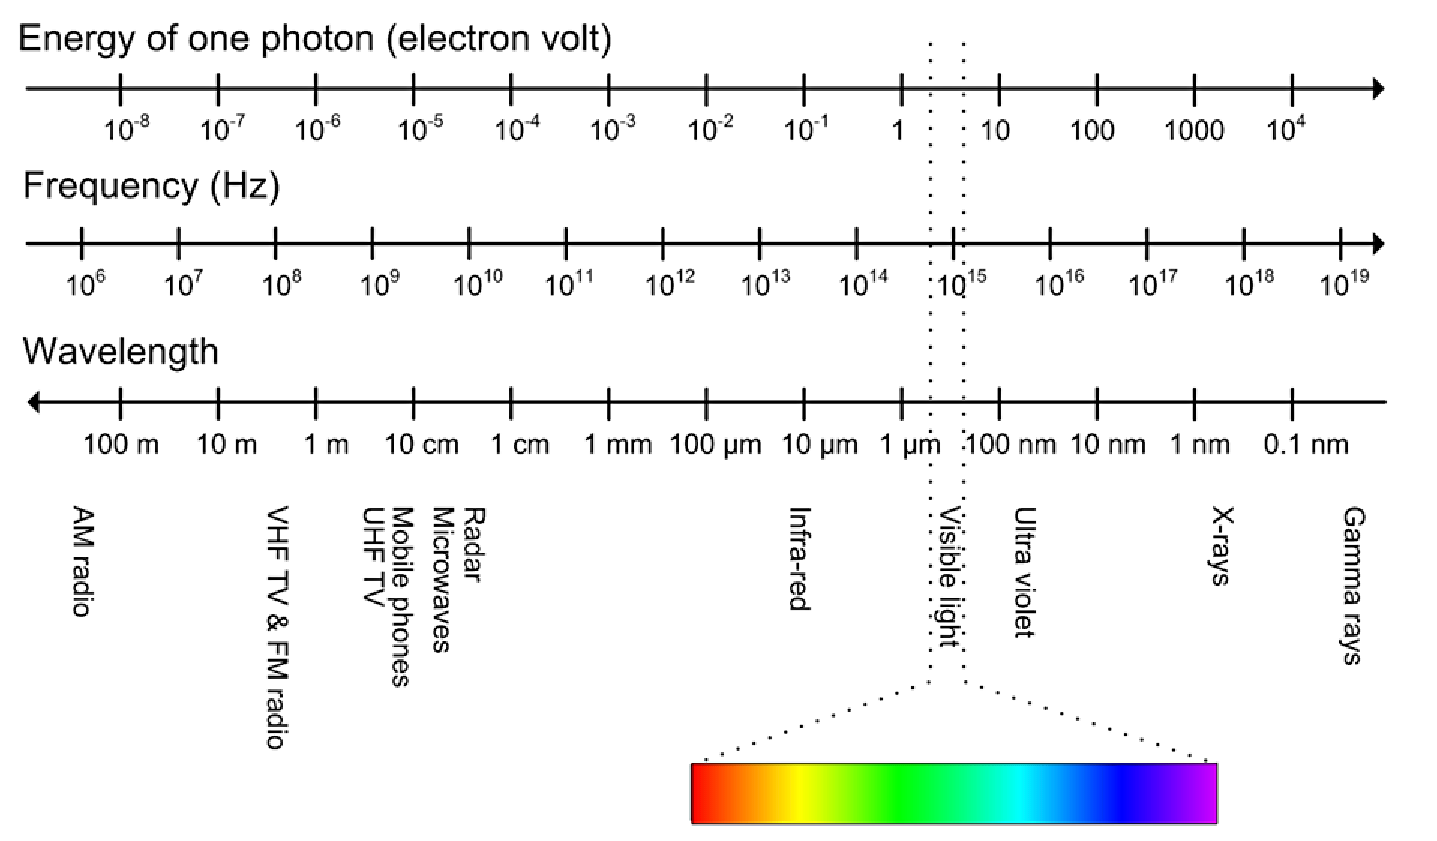
\includegraphics[width=12cm]{gfx/electromagneticSpectrum.png}
 \caption{Espectro Electromagnético \cite{Richards2009}}
 \label{fig:spectrum}
\end{figure}

Dado que la frecuencia de trabajo mayormente utilizada en este tipo de antenas comprende la región microondas del espectro
electromagnético, el cual comprende desde los 300 MHz hasta los 300 GHz (ver figura \ref{fig:spectrum}), y dado que en dicho rango la 
opacidad de la atmósfera es casi nula (ver figura \ref{fig:atmosphere}), puede decirse, en términos generales, que dichas 
antenas poseen la capacidad de trabajar independientemente de las condiciones atmosféricas. En otras palabras, la señal casi no es 
atenuada por la atmósfera, tampoco es interferida ni por las lluvias ni por las nubes. Por ejemplo, si se usa como parte de un 
radar de apertura sintética, luego de un post procesamiento de la señal recibida, es posible obtener información sobre la 
textura del terreno y sobre los sustratos inferiores de las coberturas boscosas. Dependiendo de que longitud de onda del rango de
trabajo, se tiene de 3 cm a 30 cm de penetración.

\begin{figure}[H]
 \centering
 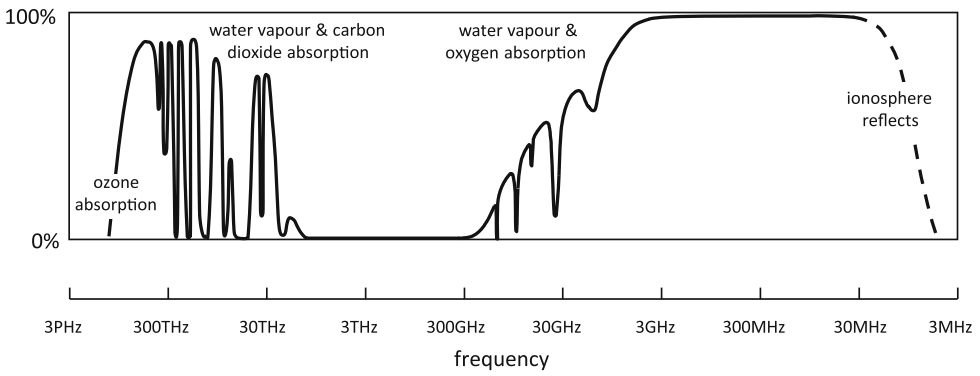
\includegraphics[width=12cm]{gfx/atmosphericOpacity.png}
 \caption{Transmisividad atmosférica en función de la frecuencia \cite{Richards2013}}
 \label{fig:atmosphere}
\end{figure}

Por convención, el eje de referencia paralelo a la dirección del recorrido del satélite es llamado azimuth y la
dirección del eje perpendicular, rango. El nadir es el punto más cercano de la tierra al satélite; en otras palabras,
es el punto en la superficie terrestre que es cortado por una recta perpendicular que también corta al satélite, ver figura
\ref{fig:antenna_ilumination}.

La antena nunca apunta directamente hacia abajo porque, de esta forma, se perdería información en rango. Al apuntar
en diagonal, y gracias a que el blanco no es puntual, el eco de la señal de la zona iluminada más cercana al nadir llega
antes al satélite que la más alejada, logrando así, tomar muestras de distintos lugares espaciados en rango (ver figura
\ref{fig:antenna_ilumination}).

\begin{figure}[H]
 \centering
 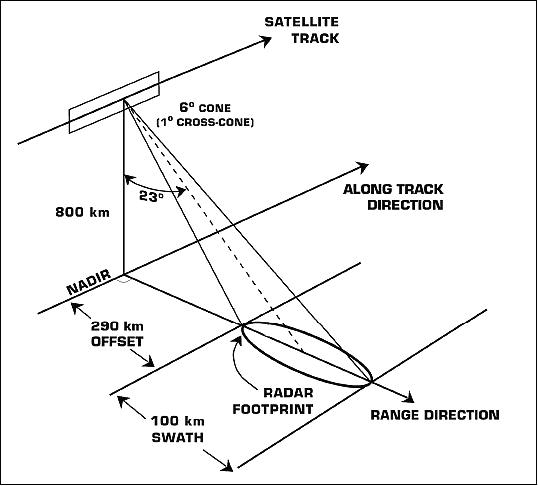
\includegraphics[width=7cm]{gfx/satellite.png}
 \caption{Pisada del satélite \cite{FootprintSatellite}.}
 \label{fig:antenna_ilumination}
\end{figure}

El tamaño de la zona iluminada se llama huella. Dicho tamaño depende tanto de las dimensiones de la antena como de la
órbita del satélite o de la altura de vuelo del avión en que está colocada dicha antena. Como se observa en la imagen
\ref{fig:footprint}, mientras más grande es la antena, más angosto es la huella, logrando así mejorar la resolución
espacial.

\begin{figure}[H]
 \centering
 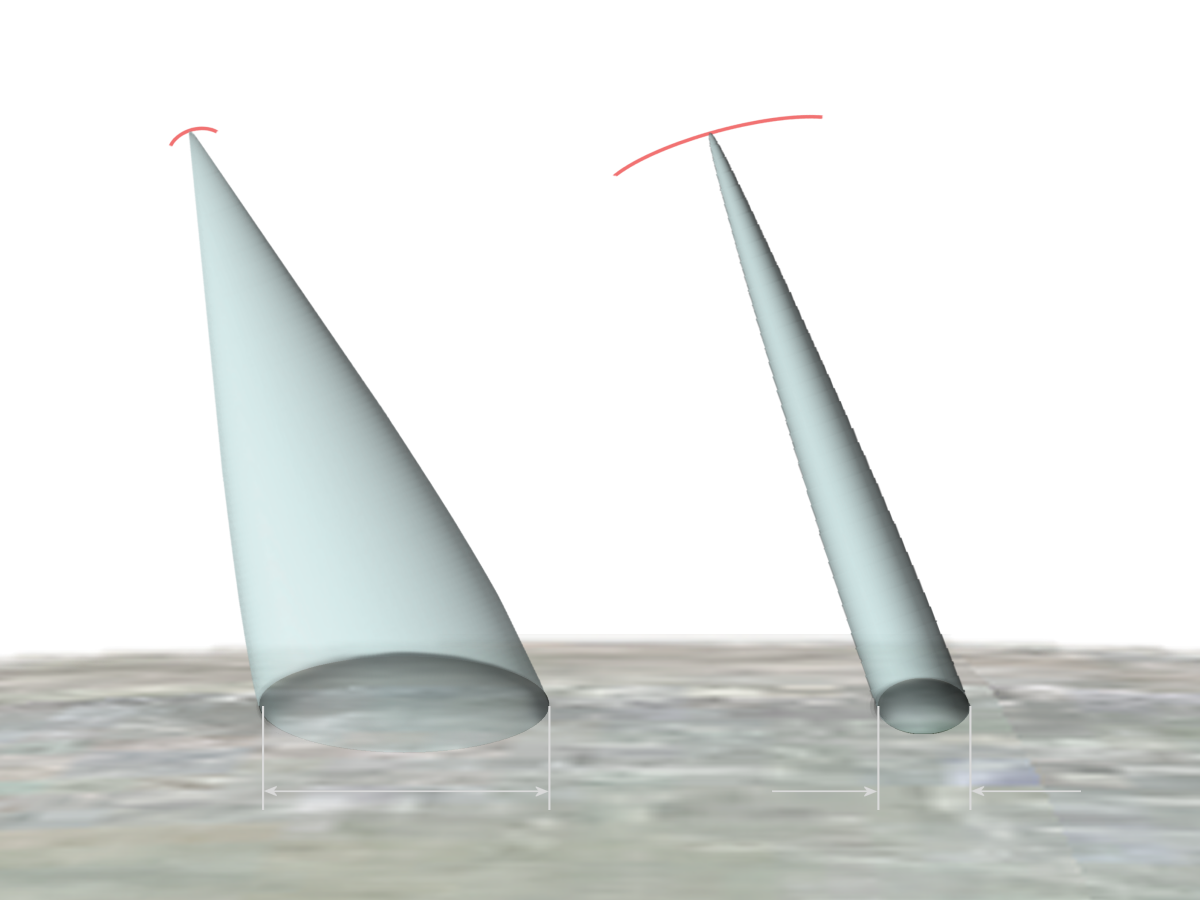
\includegraphics[width=7cm]{gfx/footprint.png}
 \caption{La huella depende del tamaño de la antena \cite{FootprintAntenna}.}
 \label{fig:footprint}
\end{figure}

\subsection{Composición de una antena}

Un conjunto de antenas en fase polarimétrica consta de una colección de $N$ elementos radiantes. Se asume que dichos elementos
poseen el mismo diagrama de radiación y que están orientados en el mismo sentido y dirección en un ambiente tridimensional. No es
necesario que estén espaciados regularmente ni que emitan los mismos valores de potencia y fase, pero si se asume
que todos están alimentados con la misma frecuencia de trabajo. En la figura \ref{fig:phasedArrayAntenna} se pueden observar
dos tipos de distribuciones comúnmente utilizadas.

\begin{figure}[H]
	\centering
 	\subfloat[]{
		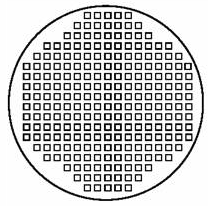
\includegraphics[width=4cm]{gfx/phasedArrayAntenna.png}}
	\subfloat[]{
		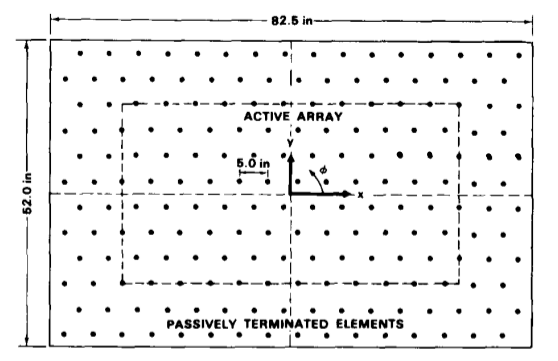
\includegraphics[width=6cm]{gfx/frontAntenna.png}}
		\caption{Conjuntos de antena: (a) Circular \cite{Bapna1996}. (b) Rectangular \cite{Aumann1989}.}
	\label{fig:phasedArrayAntenna}
\end{figure}

Este tipo de antenas está compuesto por dos bloques principales a saber: la red de distribución (o RFDN) y los elementos 
radiantes (ver figura \ref{fig:compositionAntenna}).

\begin{figure}[H]
 \centering
 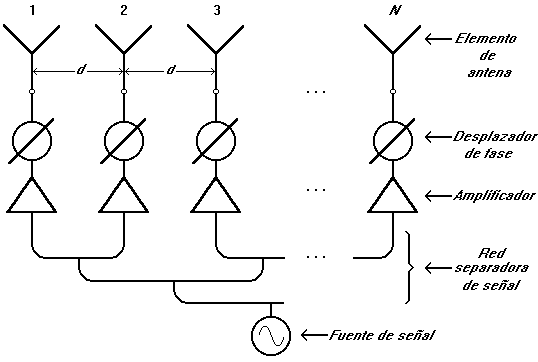
\includegraphics[width=10cm]{gfx/CompositionAntenna.png}
 \caption{Composición de un conjunto de antena con control de fase}
 \label{fig:compositionAntenna}
\end{figure}

El generador puede transmitir con distintos tipos de modulaciones. Por ejemplo cuadrada, chirp, sinusoidal, triangular. Las ventajas y
desventajas de cada una se listan en el cuadro \ref{tab:modulations}.

\begin{table}[H]
  \footnotesize
  \centering
  \begin{tabular}{|c|p{9cm}|}
	\hline
	\textbf{Modulación} & \textbf{Características} \\
	Cuadrada & Esta modulación es utilizada para mediciones muy precisas a cortas distancias comparando las fases de los dos
	semiciclos de la señal recibida. La desventaja es que los distintos ecos de los distintos blancos no pueden distinguirse.\\\hline
	Chirp & Es la modulación mayormente utilizada, se obtienen mediciones con las mayores distancias posibles.\\\hline
	Triangular & Con esta modulación se logra distinguir fácilmente la velocidad de la posición del blanco. \\\hline
	Escalonada & Es utilizada para mediciones de interferometría y para expandir el rango de medición sin ambig\"uedades.\\\hline
  \end{tabular}
  \caption{Características de cada modulación de la señal emitida}
  \label{tab:modulations}
\end{table}

La red de distribución de radio frecuencia en la antena, llamada RFDN, es la encargada de conducir la señal a todos los 
elementos radiantes de la antena. Dicha red posee una estructura de árbol, de forma tal que la longitud de todos los caminos
entre las hojas del mismo a la raíz son iguales. Los nodos son los PSC y las hojas los ERs. Es necesario que todos los caminos
sean iguales para que las señales transmitidas por defecto, es decir sin incluir el efecto de los módulos 
transmisores/receptores, tengan la misma fase y atenuación. 


\subsubsection{Identificación de los componentes de la antena}

Los componentes utilizados para distribuir la señal son los siguientes:

\begin{enumerate}
	\item Divisor/Combinador de potencia de RF: este componente es el encargado de dividir la señal transmitida en tantos puertos 
		de salida tenga y la de sumar/combinar las potencias recibidas.
	\item Cable: este componente es el utilizado para unir el resto de los componentes.
	\item Módulo de Transmisión y Recepción: Este componente es el elemento de control de fase y atenuación de la señal emitida y
		recibida por cada elemento radiante. Se modeliza que hay uno por cada elemento radiante sin embargo, la construcción y 
		diseño del modelo de antena realizado permite rápidamente adecuarlo a diferentes topologías de antena. Está compuesto por 
		los siguientes componentes de la imagen \ref{fig:compositionAntenna}:
		\begin{itemize}
			\item Desplazador de fase: Este componente desfasa la señal y es utilizado para calibrar la antena tanto en transmisión como
				en recepción, logrando así, que cada camino de Tx/Rx de las hojas a la raíz desfasen lo mismo. A su vez, se lo utiliza 
				para poder direccionar el haz de la señal emitida.
			\item Atenuador: Este componente atenúa la señal y es utilizado para calibrar la antena tanto en transmisión como en 
				recepción, logrando así que cada camino de Tx/Rx de las hojas a la raíz atenúen lo mismo. 
			\item Amplificador: Este componente es de ganancia fija y sirve para amplificar la señal tanto transmitida como recibida. 
		\end{itemize}
	\item Elemento Radiante: Este componente es el emisor de la señal a transmitir y/o el receptor. En este tipo de antenas un
		ER puede cumplir una o ambas funcionalidades.
	\item Circulador: Este componente posee tres puertos y es utilizado para separar los caminos de la señal transmitida (Tx) de 
		la recibida (Rx) cuando un mismo elemento radiante posee las funcionalidades de transmisión y recepción. 
\end{enumerate}

Se pueden conectar los elementos radiantes de tal forma que puedan transmitir en dos polarizaciones distintas, H y V, para esto,
se debe duplicar la RFDN. Haciendo uso de ambas polarizaciones se puede caracterizar los blancos observados, dado que, cada
cuerpo responde de forma distinta a cada tipo de polarización.

\subsection{Diagrama de radiación de antena}

Un conjunto de antena puede armarse recursivamente, esto es, que un elemento sea, en sí mismo, un conjunto. Un diagrama de antena es
un diagrama de radiación polar que resulta de reemplazar cada elemento por un radiador isótropo. Si se asume que el diagrama de
radiación de cada elemento es idéntico al del resto, tomando una cierta incertidumbre, el diagrama de radiación total resulta de
la multiplicación de todos los diagramas de todos los elementos. Este resultado no depende de si se consideran los diagramas de
potencia o de amplitud/fase. 

\begin{figure}[H]
 \centering
 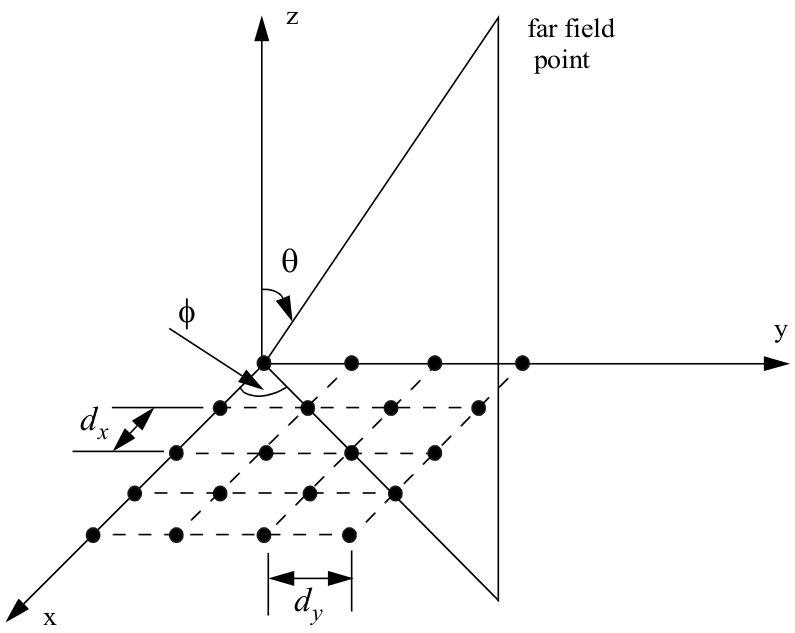
\includegraphics[width=7cm]{gfx/rectangularArrayGeometry.png}
 \caption{Conjunto de geometría rectangular \cite{Mahafza2004}}
 \label{fig:arrayGeometry}
\end{figure}

Considérese un conjunto de antena de $N$ por $M$ elementos, como se muestra en la figura \ref{fig:arrayGeometry}, el diagrama de
radiación de campo lejano se lo calcula de la siguiente forma \cite{Mahafza2004}.
\begin{equation}
	E(\theta, \phi) = \sum_{n=0}^{N-1}\sum_{m=0}^{M-1} I_{n,m} e^{jk(d_xn\sin\phi\cos\theta + d_ym\sin\phi\sin\theta)}
\end{equation}
Donde $\theta$ corresponde al ángulo al eje x, $\phi$ corresponde al ángulo al eje $z$, $k$ es el número de onda y es igual
a $2\pi/\lambda$, $I_{n,m}$ es la amplitud compleja del elemento $n,m$. La figura \ref{fig:arrayPattern} muestra el diagrama de
radiación en tres dimensiones, donde el eje $z$ (representado con colores) es la potencia radiada. A su vez, se puede apreciar 
el corte horizontal del mismo.

\begin{figure}[H]
 \centering
	\subfloat[]{
		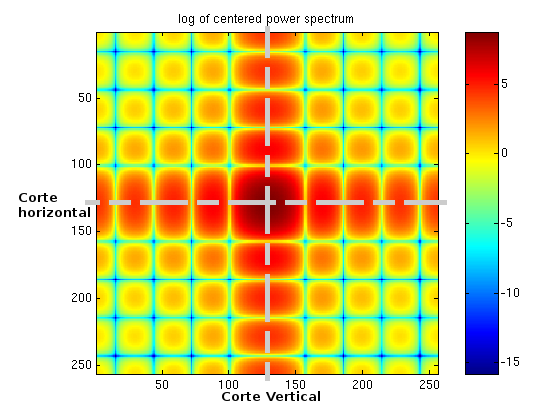
\includegraphics[width=7cm]{gfx/arrayPattern3D.png}}
 	\subfloat[]{
		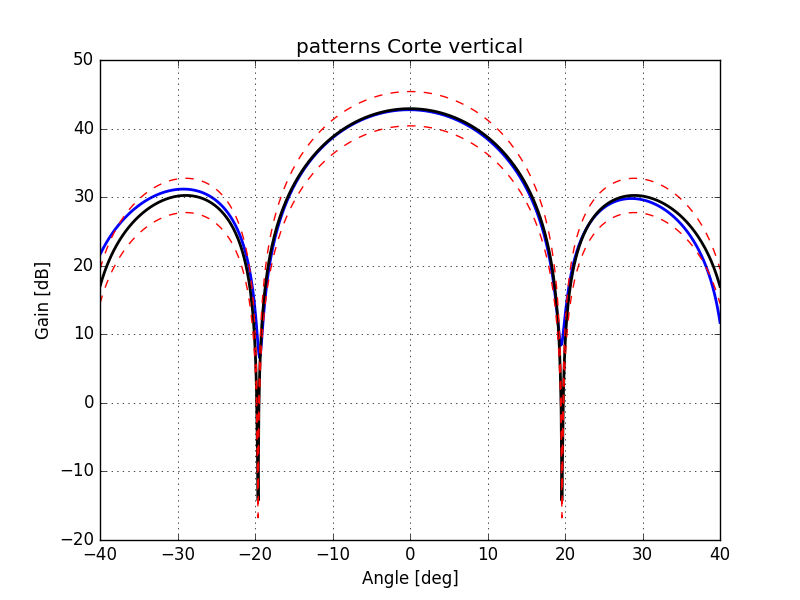
\includegraphics[width=7cm]{gfx/arrayPatternCut.png}}
	\caption{diagramas de radiación de un conjunto de antena (a) diagrama en 3 dimensiones \cite{arrayPattern} (b) corte horizontal}
 \label{fig:arrayPattern}
\end{figure}

Tres parámetros importantes del diagrama de radiación son la directividad, el ancho del lóbulo principal y el nivel de los
lóbulos secundarios \cite{Hsiao1985}, estos 3 parámetros tienen incidencia directa en el apuntamiento. Es importante incrementar
lo más posible la diferencia de potencia entre los lóbulos secundarios y el principal porque los lóbulos secundarios apuntan
en distintas direcciones a la deseada brindando así información de un punto indeseado. Como son variables dependientes entre
sí, si se desea realizar una reducción de los lóbulos secundarios sin modificar la directividad como el ancho del lóbulo 
principal, es necesario incrementar el tamaño del conjunto de antena \cite{Hsiao1985}. 
Lamentablemente los errores, incertidumbres y desvíos en el comportamiento del conjunto limitan los niveles que se pueden 
obtener de los lóbulos secundarios \cite{Hsiao1985}.

A continuación se muestran gráficos representando la potencia del campo radiado, asumiendo campo lejano. La potencia decae
con la relación de $1/r$, donde $r$ es la distancia del punto de medición al elemento radiado. Se debe tomar en cuenta también
la fase con que emite el elemento y el retardo de fase que se debe a la distancia recorrida por la señal para llegar a los 
distintos lugares del espacio. Dicho retardo es expresado como $2\pi r/\lambda$, siendo $\lambda$ la longitud de onda de la 
señal emitida por el elemento radiado. Los gráficos \ref{fig:twoArrayPat} y \ref{fig:fourArrayPat} muestran las curvas de 
nivel de diagramas de radiación de potencia polar, donde los elementos radiantes están distribuidos uniformemente sobre el eje
x (eje horizontal) y emiten en fase.

\begin{figure}[H]
	\centering
	\subfloat[]{
		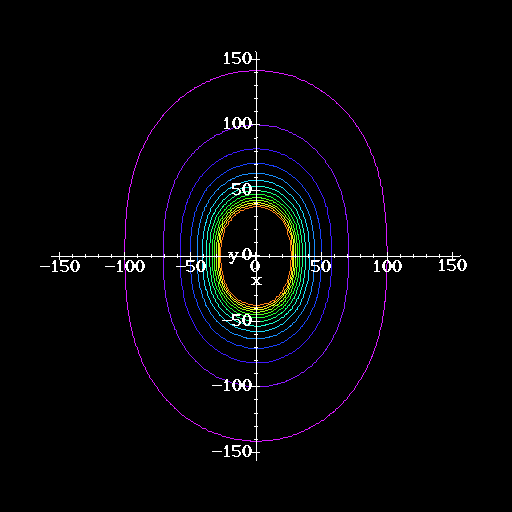
\includegraphics[width=5cm]{gfx/TwoIsoQuartDist.png}}
	\subfloat[]{
		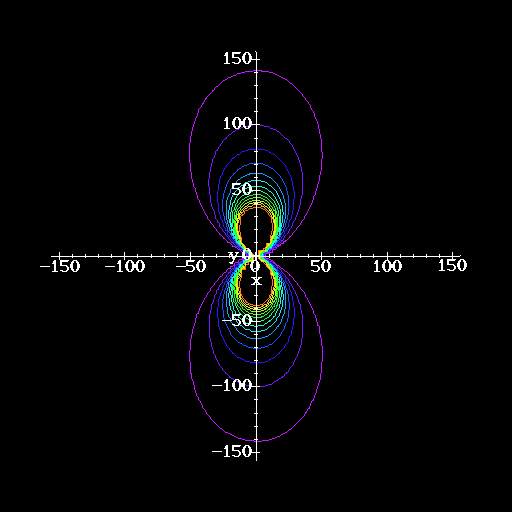
\includegraphics[width=5cm]{gfx/TwoIsoHalfDist.png}}
	\caption{Diagramas de radiación de potencia. Dos ERs con separación de: a) $1/4$ de longitud de onda, b) $1/2$ de longitud de onda}
	\label{fig:twoArrayPat}
\end{figure}

\begin{figure}[H]
	\centering
	\subfloat[]{
		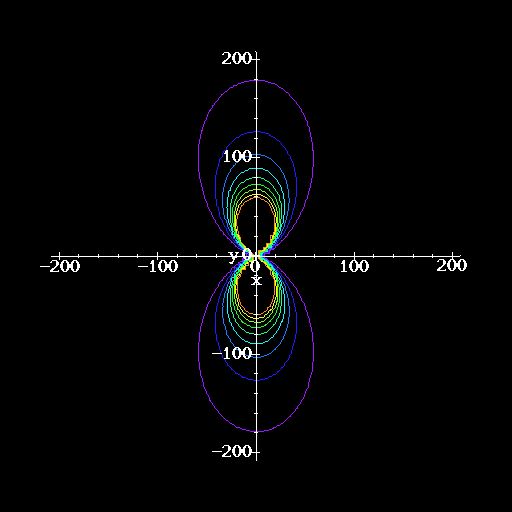
\includegraphics[width=5cm]{gfx/FourIsoQuartDist.png}}
	\subfloat[]{
		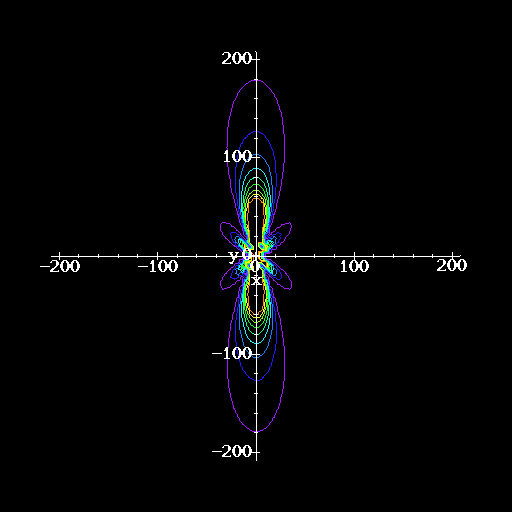
\includegraphics[width=5cm]{gfx/FourIsoHalfDist.png}}
	\caption{Diagramas de radiación de potencia. Cuatro ERs con separación de: a) $1/4$ de longitud de onda, b) $1/2$ de longitud
		de onda}
	\label{fig:fourArrayPat}
\end{figure}

Se puede observar que aumentando la cantidad de elementos radiantes, se logra que el haz principal (lóbulo principal de
potencia) sea más angosto, por lo tanto se obtenga una mayor resolución del cuerpo observado. 

La figura \ref{fig:directArrayPat} muestra que la fase con que emiten los elementos radiados modifica el apuntamiento de la 
antena.

\begin{figure}[H]
	\centering
	\subfloat[]{
		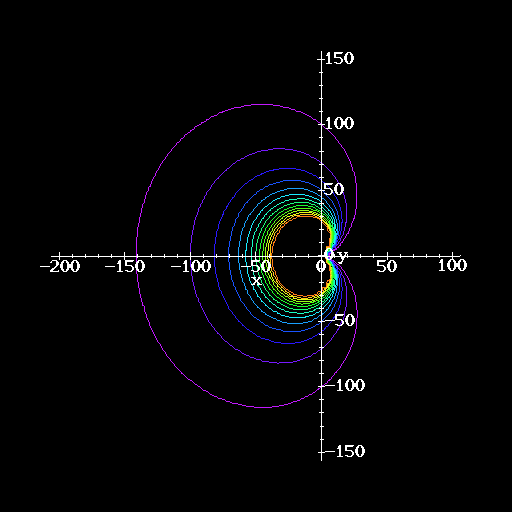
\includegraphics[width=5cm]{gfx/TwoQuarterPhase.png}}
	\subfloat[]{
		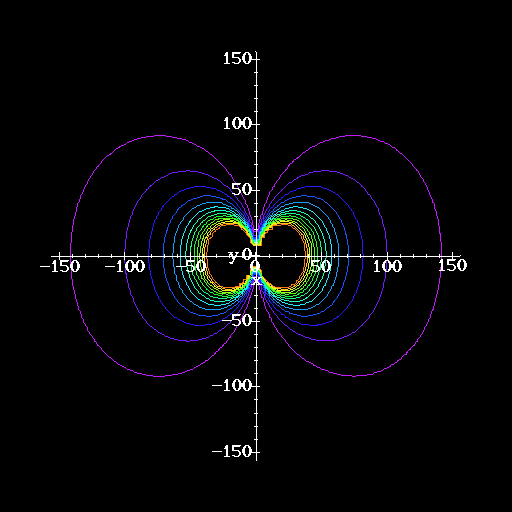
\includegraphics[width=5cm]{gfx/TwoAntiPhase.png}}
	\caption{Diagrama de radiación de potencia. Dos ERs en contrafase y con separación de: a) $1/4$ de longitud de onda. b) $1/2$ 
		de longitud de onda}
	\label{fig:directArrayPat}
\end{figure}


\subsection{Apuntamiento de una antena}\label{ssec:beamSteering}

Para que la suma de las señales emitidas con todos los elementos radiantes apunte a un mismo punto, es necesario que
todas las ondas lleguen al objetivo con la misma fase. Por esto se debe poder determinar cual es la fase individual que
debe tener cada uno de los elementos radiantes.

Como primer simplificación, se puede asumir que todas las rectas de cada uno de los elementos radiantes al punto lejano son
paralelas entre ellas. A su vez, como el camino recorrido desde cada elemento radiante al punto lejano es diferente, es
necesario calcular dicha diferencia para luego relacionarla con la fase. De esta forma, se puede retrasar la fase emitida de
los elementos más alejados al punto para que todas las señales lleguen en fase, logrando así, una onda plana. La figura 
\ref{fig:beamSteering} muestra un ejemplo de un apuntamiento de un conjunto de antena.

\begin{figure}[H]
 \centering
 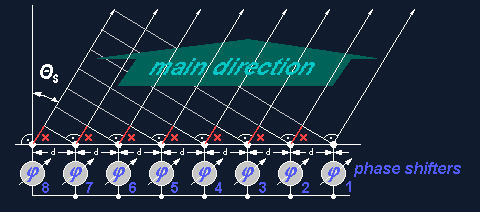
\includegraphics[width=10cm]{gfx/beamSteering.png}
 \caption{Apuntamiento con un conjunto de antena \cite{BeamSteering}.}
 \label{fig:beamSteering}
\end{figure}

Como se puede observar en la figura \ref{fig:beamSteering}, la diferencia de fase entre dos elementos consecutivos,
$\Delta\varphi$, es constante y es llamada incremento de fase \cite{BeamSteering}. Se la puede relacionar con la diferencia
de distancia que tiene que recorrer el haz emitido por cada elemento radiante. Dicha diferencia de distancia se la calcula con
la siguiente relación matemática,


\begin{equation}
	x = d\cdot \sin{\theta_s}
	\label{eq:steering}
\end{equation}
Donde $d$ es la distancia entre dos elementos consecutivos y $\theta_s$ es el apuntamiento deseado del haz emitido. Para calcular
el desfase de una onda en una cierta distancia $x$, se debe tener en cuenta que depende de su longitud de onda.

\begin{equation}
	\dfrac{2\pi}{\Delta\varphi} = \dfrac{\lambda}{x}
	\label{eq:dist2angle}
\end{equation}
Donde $\Delta\varphi$ es el incremento de fase entre elementos radiantes, $\lambda$ es la longitud de onda transmitida.
Utilizando las ecuaciones \ref{eq:steering} y \ref{eq:dist2angle} se puede obtener el incremento de fase entre ERs contiguos 
necesario para cumplir con el apuntamiento deseado. La ecuación a continuación.

\begin{equation}
	\Delta\varphi = \dfrac{2\pi\cdot d\cdot\sin{\theta_s}}{\lambda}
\end{equation}

\subsection{Calibración interna de una antena polarimétrica}

La respuesta de los componentes en el tiempo no se mantiene invariante. Hay diversos factores que influyen en su comportamiento a
medida que transcurre su vida útil. Por un lado su envejecimiento natural por el uso. Por otro lado las variaciones en su 
comportamiento por efectos de temperatura. En algunos casos, cuando se trata de componentes activos, el desgaste que pueden
sufrir de manera acelerada por superar niveles de derating. Dichas variaciones deben ser corregidas, buscando que no solo todos
los caminos de recepción atenúen y desfasen exactamente lo mismo, sino que también sea un valor conocido. En transmisión el
objetivo es el mismo, con la salvedad que se busca que cada TRM trabaje en su punto de compresión (generalmente cerca de los
6 dB) y que la fase de cada elemento depende del apuntamiento deseado.

Para poder corregir las variaciones en transmisión y recepción de la antena, se hace uso de actuadores. En la presente tesis,
estos componentes fueron modelados como TRMs, los cuales, pueden introducir fase y atenuación en el sistema a elección, con
cierta incertidumbre. Por ejemplo, en la figura \ref{fig:antennaTRM} se observa un esquema 
de conexionado de una antena en transmisión donde el TRM se encuentra resaltado.

\begin{figure}[H]
 \centering
 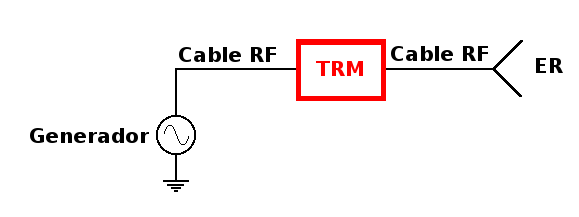
\includegraphics[width=10cm]{gfx/antennaTRM.png}
 \caption{Esquema de transmisión de una antena.}
 \label{fig:antennaTRM}
\end{figure}

La antena está conectada a la unidad central de control, dispositivo que posee numerosas funciones, las relevantes a la presente tesis 
son:
\begin{enumerate}
	\item Desde el punto de vista de RF: se comporta como un VNA en cuanto a que transmite (tiene un generador) y escucha (tiene un
		receptor).
	\item Desde el punto de vista digital y de control: se comporta como una computadora central indicando la fase y atenuación que
		cada TRM debe introducir, que no necesariamente es la de salida de los ERs.
\end{enumerate}

Para calibrar la antena por medio de lazos de calibración, la unidad central de control emite una señal por un canal y la 
compara con lo recibido en el otro canal, midiendo el S21 (transmisión directa) de los parámetros S de la antena. Para ello, se
debe descontar a la señal recibida, la señal emitida. Dicha calibración determina las características de la antena para un
determinado instante, si los componentes cambian sus características en el tiempo, se debería realizar el proceso de
calibración nuevamente para obtener los nuevos parámetros S.

La figura \ref{fig:calibrationLoop} muestra un esquema de calibración en donde el lazo está compuesto por dos antenas y, como
todos los elementos que pueden influenciar en la fase y amplitud de la señal que se transmite quedan dentro del lazo de 
calibración, se pueden medir las variaciones de la señal recibida y, si hubiese un TRM, se las podrían corregir.

\begin{figure}[H]
 \centering
 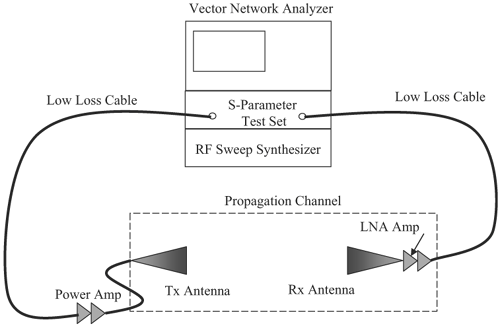
\includegraphics[width=10cm]{gfx/calibrationLoop.png}
 \caption{Lazo de calibración utilizando un VNA \cite{Reed2012}.}
 \label{fig:calibrationLoop}
\end{figure}

En caso que hayan componentes que puedan influenciar en la fase y atenuación transmitida por la antena fuera del lazo de
calibración, al calibrar el sistema no se podrá medir correctamente la transferencia del sistema, por lo tanto, no se podrán
corregir completamente las variaciones de la misma. Para acotar este error, se deben caracterizar los componentes que están
fuera del lazo asumiendo que dichas caracterizaciones son válidas para toda la vida útil de los mismos.

La figura \ref{fig:nonCalPattern} muestra la comparación de dos diagramas de radiación de antena, uno calibrado e ideal y el
otro sin calibrar. Se puede observar como los niveles de los lóbulos secundarios y el ancho del lóbulo principal se incrementan.

\begin{figure}[H]
 \centering
 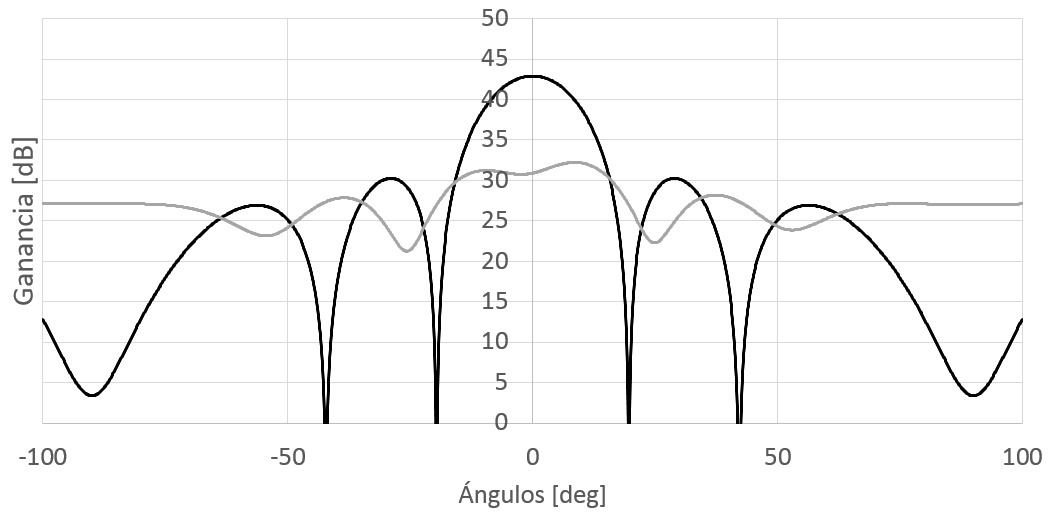
\includegraphics[width=10cm]{gfx/nonCalPattern.png}
 \caption{Diagrama de radiación de antena calibrado vs no calibrado.}
 \label{fig:nonCalPattern}
\end{figure}


\section{Desarrollo del modelo de antena en parámetros S}

Los componentes que son ideales, se los trata como si estuviesen perfectamente adaptados, logrando así que los coeficientes
de reflexión sean nulos, esto es $S_{11} = S_{22} = 0$. 


\subsection{Elemento Radiante (ER)}

Las antenas utilizadas como elementos radiantes en un conjunto de antena son los dipolos y monopolos \cite{Balanis2012}, en esta
tesis se modelará un monopolos como ER, ver figura \ref{fig:radiatingElement}.
\begin{figure}[H]
	\centering
	\subfloat[Rectangular]{
		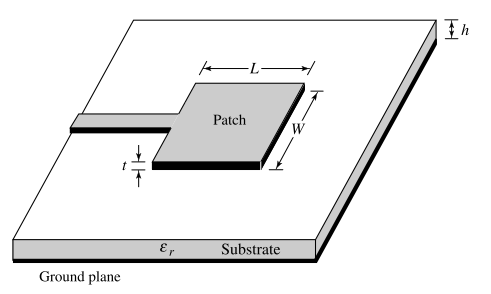
\includegraphics[width=6cm]{gfx/rectangularPatch.png}}
	\subfloat[Circular]{
		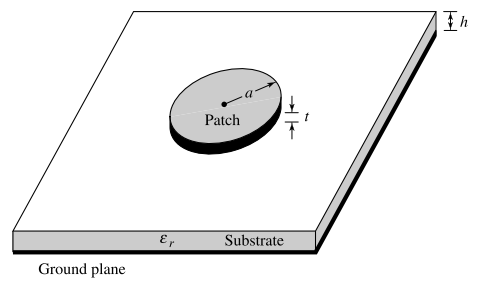
\includegraphics[width=6cm]{gfx/circularPatch.png}}
		\caption{Antenas monopolo circulares y cuadradas \cite{Balanis2012}.}
	\label{fig:radiatingElement}
\end{figure}

El elemento radiante es un módulo de un único puerto y es pasivo, por lo tanto el parámetro S que lo define es $S_{11}$ y su
valor varía entre -1 y 1.

\begin{itemize}
	\item Cortocircuito ideal: $S_{11} = -1$
	\item Conexión ideal: $S_{11} = 0$
	\item Circuito abierto ideal: $S_{11} = 1$
\end{itemize}

Los casos de cortocircuito y circuito abierto son casos de falla del módulo radiante. Cualquier otro valor intermedio implica
una desadaptación de impedancias.

\subsection{Cable ideal}
El cable de RF es el dispositivo utilizado para interconectar el resto de los componentes, en la presente tesis puede no ser 
utilizado dado que es configurable. La figura \ref{fig:cableRF} muestra un típico cable utilizado en aplicaciones espaciales 
para frecuencias de $32GHz$ \cite{Gore2013}.

\begin{figure}[H]
 \centering
 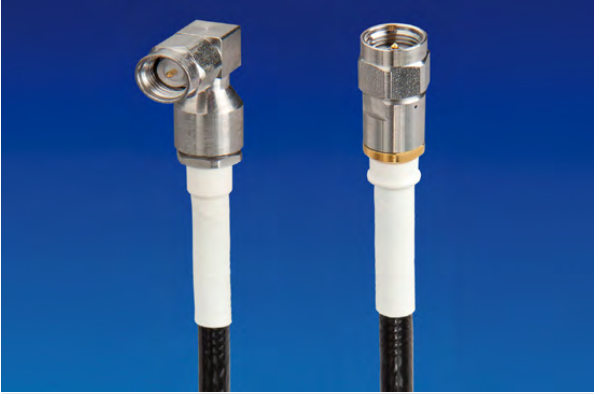
\includegraphics[width=5cm]{gfx/cableRF.png}
 \caption{Cable de RF \cite{Gore2013}.}
 \label{fig:cableRF}
\end{figure}

Como un cable se comporta como una línea de transmisión, se propone la siguiente matriz de parámetros S que la 
representa.

$$
\mathbf{S} = \begin{pmatrix} 0 & e^{-\gamma l}\\e^{-\gamma l} & 0\end{pmatrix}
$$
Donde $\gamma = \alpha + j\beta$ es una constante de propagación compleja. $\alpha$ es la atenuación de la línea en [neper/m]
y $\beta = 2\pi/\delta$ con la longitud de onda $\delta$. Para una línea sin pérdidas se obtiene $|S_{21}| = 1$

\subsection{Desplazador de fase ideal}

Un desplazador de fase ideal modifica la fase de una señal periódica con respecto a una referencia \cite{Standard1996}. El 
desfase puede ser fijo o ajustable de forma continua o incremental. La imagen \ref{fig:phaseShifter} muestra un desfasador 
controlado por tensión.

\begin{figure}[H]
 \centering
 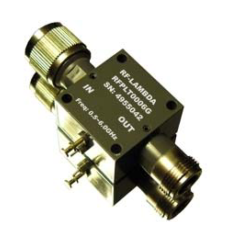
\includegraphics[width=4cm]{gfx/phaseShifter.png}
 \caption{desplazador de fase ajustable por tensión \cite{Shifter}}
 \label{fig:phaseShifter}
\end{figure}

En la presente tesis se modeliza un desplazador de fase con desfase ajustable de forma continua, por lo tanto se propone la 
siguiente matriz de parámetros S.

$$
\mathbf{S} = \begin{pmatrix} 0 & e^{-j\phi_{12}}\\e^{-j\phi_{21}} & 0\end{pmatrix}
$$

Un defasador recíproco posee $\phi_{12} = \phi_{21}$.

\subsection{Atenuador ideal}

Un atenuador ideal reduce la amplitud de una señal sin una distorsión apreciable en su forma de onda. La atenuación puede ser
fija o ajustable de forma continua o incremental \cite{Standard1996}. La atenuación se la expresa en decibeles relativos a la
potencia. La imagen \ref{fig:attenuator} muestra un atenuador fijo de $10 dB$.

\begin{figure}[H]
 \centering
 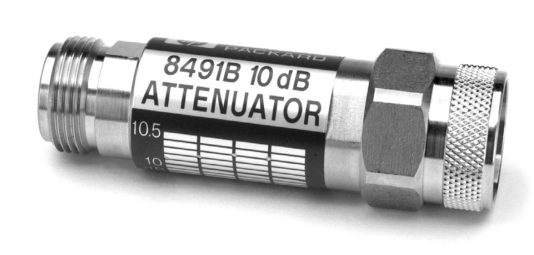
\includegraphics[width=4cm]{gfx/attenuator.png}
 \caption{atenuador fijo de 10 dB \cite{Keysight2014}}
 \label{fig:attenuator}
\end{figure}

En la presente tesis se modeliza un atenuador con atenuación ajustable de forma continua, por lo tanto se propone la siguiente
matriz de parámetros S para representarlo.

$$
\mathbf{S} = \begin{pmatrix} 0 & e^{-\beta}\\e^{-\alpha} & 0\end{pmatrix}
$$

Si el atenuador es recíproco, $\alpha = \beta$. El factor de atenuación $\alpha$ es expresado en neper, donde $1N = 8.686dB$.
La atenuación en decibeles viene dado por $A = 20\log_{10}(S_{21})$. 


\subsection{Amplificador ideal}

Un amplificador ideal incrementa la amplitud de una señal sin una distorsión apreciable en su forma de onda. La ganancia puede
ser fija o ajustable de forma continua o incremental \cite{Standard1996} y es en una única dirección, del puerto de entrada al
de salida. En la dirección opuesta la ganancia es 0, implica una atenuación infinita. La imagen \ref{fig:amplifier} muestra un
amplificador fijo de $40 dB$.

\begin{figure}[H]
 \centering
 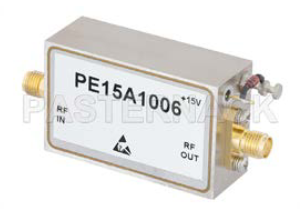
\includegraphics[width=4cm]{gfx/amplifier.png}
 \caption{amplificador fijo de 40 dB \cite{Pasternack2014}}
 \label{fig:amplifier}
\end{figure}

En la presente tesis se modeliza un amplificador con ganancia fija, por lo tanto se propone la siguiente matriz de parámetros S
para representarlo.

$$
\mathbf{S} = \begin{pmatrix} 0 & 0\\G & 0\end{pmatrix}
$$

Con $G > 1$ fijo.


\subsection{Módulo de transmisión recepción ideal}

Dicho componente está compuesto por un desfasador ideal junto a un amplificador y un atenuador. Es un componente de tres puertos,
el primero puede transmitir o recibir señal, el segundo solamente transmitir y el tercero recibir. Su matriz de parámetros S es
la siguiente.

$$
	S_{PSC} = \begin{pmatrix} 0&0&Ge^{-j\phi_{13}} \\ Ge^{-j\phi_{21}}&0&0 \\ 0&0&0\end{pmatrix} 
$$

Este componente se lo puede configurar para unir el primer puerto con el segundo o con el tercero por medio de un interruptor, 
por lo tanto no se lo puede utilizar para transmitir y recibir a la vez. 

\begin{figure}[H]
 \centering
 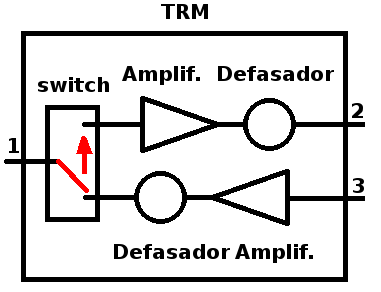
\includegraphics[width=6cm]{gfx/trm.png}
 \caption{módulo de transmisión/recepción}
 \label{fig:trm}
\end{figure}


\subsection{Circulador ideal}

El circulador ideal es sin pérdidas y adaptado en todos sus puertos. La señal entrante por un puerto es exclusivamente
transmitida al puerto siguiente en el sentido de las flechas.

\begin{figure}[H]
	\centering
 	\subfloat[Circulador de tres puertos ]{
		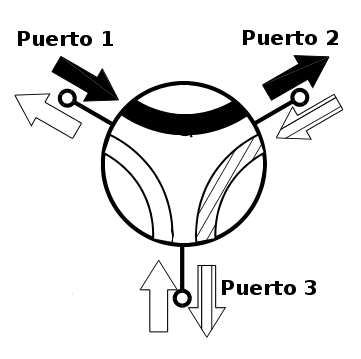
\includegraphics[width=5cm]{gfx/3PortsCirculator.png}}
	\subfloat[Circulador de cuatro puertos]{
		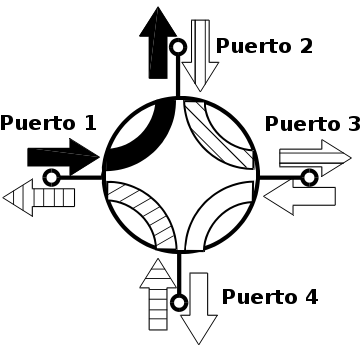
\includegraphics[width=5cm]{gfx/4PortsCirculator.png}}
	\caption{flujo de energía en circuladores \cite{Semiconductors1998}.}
	\label{fig:circulator}
\end{figure}

En la presente tesis se modelizan circuladores de tres puertos proponiendo la siguiente matriz de parámetros S.

$$
\mathbf{S} = \begin{pmatrix} 0 & 0 & 1\\1 & 0 & 0\\0 & 1 & 0\end{pmatrix}
$$


\subsection{Divisor/Combinador de potencia en RF (PSC)}

El tipo de PSC modelado consiste en una red recíproca y adaptada en todos sus puertos, pero con pérdidas. Puede ser un
componente de 3 o más puertos. Como ejemplo, en la figura \ref{fig:3PortsPSC} se muestra un PSC de 3 puertos. Al utilizarlo como
divisor de potencia, se aplica una señal en el puerto S y se obtiene la misma señal atenuada en los puertos A y B. Cuando es
utilizado como combinador, se aplican señales en los puertos A y B y la suma es obtenida en el puerto S \cite{MiniCircuits2015}.

\begin{figure}[H]
 \centering
 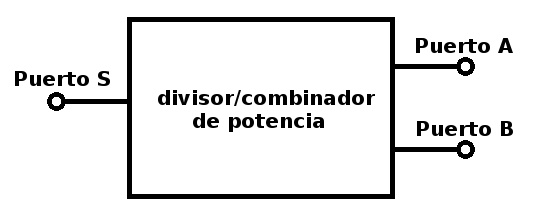
\includegraphics[width=7cm]{gfx/3PortsPSC.png}
 \caption{PSC de tres puertos \cite{MiniCircuits2015}.}
 \label{fig:3PortsPSC}
\end{figure}

En la presente tesis, como es configurable la cantidad de puertos totales de los PSC utilizables en el modelo de antena, se 
propone la siguiente matriz de parámetros S genérica de n puertos.

$$
\mathbf{S} = \begin{pmatrix} 0 & \dfrac{1}{n-1} & ... & \dfrac{1}{n-1}\\
							 \dfrac{1}{n-1} & 0 & ... & \dfrac{1}{n-1}\\
							 ... & ... & ... & ... \\
							 \dfrac{1}{n-1} & \dfrac{1}{n-1} & ... & 0 \end{pmatrix}
$$

\subsection{Acoplamientos mutuos}

El acoplamiento mutuo entre módulos radiantes es modelizado con el mismo comportamiento al de un cable, pero con las
propiedades de atenuación y desfase de una onda en \enquote*{espacio libre}. Las cuales son:

\begin{equation}
	S12 = S21 = \dfrac{e^{-j\frac{\pi}{\lambda}r}}{4\pi r^2}
\end{equation}

siendo r la distancia recorrida por la señal. La matriz de parámetros S resulta,

$$
\mathbf{S} = \begin{pmatrix} 0 & \frac{e^{-j\frac{\pi}{\lambda}r}}{4\pi r^2}\\\frac{e^{-j\frac{\pi}{\lambda}r}}{4\pi r^2} & 0\end{pmatrix}
$$

\section{Sistema interconectado básico en parámetros S, para una polarización}

En esta sección se ejemplifica el armado de las matrices de parámetros S de la antena en una sola polarización desde el punto 
de transmisión a cada elemento radiante. Se asume que se tiene una antena de dos elementos radiantes con la configuración de 
RFDN de la figura \ref{fig:antennaS}. Dicha figura muestra solamente la red de distribución en una sola polarización, para la 
otra polarización, este esquema se repite.

\begin{figure}[H]
 \centering
 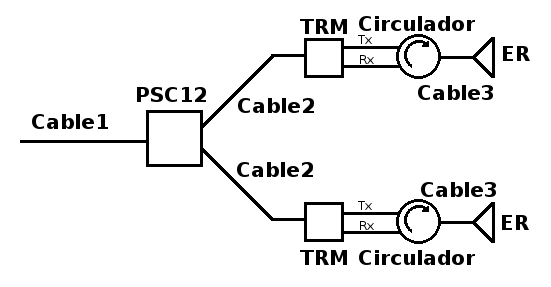
\includegraphics[width=9cm]{gfx/RFDN.png}
 \caption{RFDN para una polarización del esquema de antena.}
 \label{fig:antennaS}
\end{figure}

La tabla \ref{tab:componentSParameters} muestra la cantidad de puertos que posee cada componente y la conexión de cada puerto.

\begin{table}[H]
  \footnotesize
  \centering
  \begin{tabular}{|c|c|p{6cm}|}
	\hline
	\textbf{Componente de Antena} & \textbf{Cantidad de puertos} & \textbf{Notas} \tabularnewline \hline
	cable1 &  2 & Permite interconectar la electrónica de la Unidad Central de Control con el PSC12 \tabularnewline \hline
	\multirow{3}{*}{PSC12} & & Puerto1: conexión cable1 \tabularnewline
	 & 3 & Puerto2: conexión Cable2 (superior) \tabularnewline
	 & & Puerto3: conexión Cable2 (inferior) \tabularnewline \hline
	Cable2 & 2 & \tabularnewline \hline
	\multirow{3}{*}{TRM} & & Puerto1: conexión cable2 \tabularnewline
	 & 3 & Puerto2: conexión Tx \tabularnewline
	 & & Puerto3: conexión Rx \tabularnewline \hline
	\multirow{3}{*}{Circulador} & & Puerto1: conexión Tx \tabularnewline
	 & 3 & Puerto2: conexión Cable3 \tabularnewline
	 & & Puerto3: conexión Rx \tabularnewline \hline
	Cable3 & 2 & Permite interconectar el Circulador al Elemento Radiante \tabularnewline \hline
	ER & 1 &   \tabularnewline \hline
  \end{tabular}
  \caption{Propiedades físicas de cada componente de una antena}
  \label{tab:componentSParameters}
\end{table}

Para la obtención de la respuesta del sistema desde el punto de transmisión/recepción a cada elemento radiante se debe
transformar las matrices de 3 puertos en matrices de 2 puertos. Asumiendo que se desea obtener la respuesta del sistema de
transmisión del elemento radiante 2, camino con trazo más grueso de la figura \ref{fig:antennaSLoop}, quedan definidos los puertos de
conexión para la transformación de dichas matrices.

\begin{figure}[H]
 \centering
 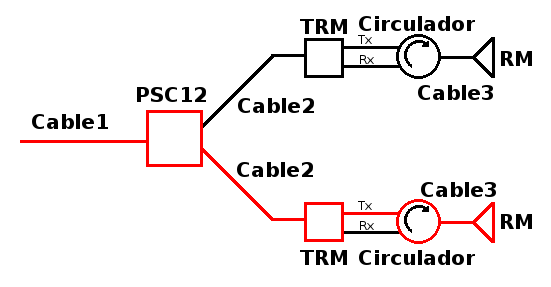
\includegraphics[width=9cm]{gfx/RFDNLoop.png}
 \caption{RFDN para una polarización del esquema de antena. Trazo grueso, cascada de redes de dos puertos.}
 \label{fig:antennaSLoop}
\end{figure}

Es importante aclarar que las variables de cada matriz de parámetros S poseerán la nomenclatura $S_{ij}$, siendo $i,j$ la
posición en fila/columna de la variable en dicha matriz. A su vez, cada $S_{ij}$ es diferente entre las distintas matrices. 

Como los puertos utilizados por el PSC en el camino rojo de la figura \ref{fig:antennaSLoop} son el 1 y 3, la conversión de
parámetros S resulta ser,

$$
	S_{PSC} = \begin{pmatrix} S11&S12&S13 \\ S21&S22&S23 \\ S31&S32&S33\end{pmatrix} \Rightarrow
	S_{PSC_{13}} = \begin{pmatrix} S11&S13 \\ S31&S33 \end{pmatrix}
$$

Los puertos utilizados por el TRM, indicados en la figura \ref{fig:antennaSLoop} y en la tabla \ref{tab:componentSParameters},
son el 1 y 2. 

$$
	S_{TRM} = \begin{pmatrix} S11&S12&S13 \\ S21&S22&S23 \\ S31&S32&S33\end{pmatrix} \Rightarrow
	S_{TRM_{12}} = \begin{pmatrix} S11&S12 \\ S21&S22 \end{pmatrix}
$$

Los puertos utilizados por el circulador, indicados en la figura \ref{fig:antennaSLoop} y en la tabla \ref{tab:componentSParameters},
también son el 1 y 2. 

$$
	S_{Circulador} = \begin{pmatrix} S11&S12&S13 \\ S21&S22&S23 \\ S31&S32&S33\end{pmatrix} \Rightarrow
	S_{Circulador_{12}} = \begin{pmatrix} S11&S12 \\ S21&S22 \end{pmatrix}
$$

Como se desea caracterizar la respuesta de una cascada de redes de dos puertos, se transforman todas las matrices de cada
componente a parámetros T (ver ecuaciones \ref{eq:s2t}), se multiplican todas las matrices como se muestra en la ecuación
\ref{eq:cascade} y luego, la matriz resultante se la vuelve a convertir a parámetros S (ver ecuaciones \ref{eq:t2s}).

$$
\begin{aligned}
	S_i &\Rightarrow T_i \\
	T_{in,rm2} &= T_{Cable1}\cdot T_{PSC_{13}}\cdot T_{Cable2}\cdot T_{TRM_{12}}\cdot T_{Circulador_{12}}\cdot T_{Cable3}\cdot T_{RM}\\
	T_{in,rm2} &\Rightarrow S_{in,rm2}
\end{aligned}
$$

Para el caso de querer caracterizar la respuesta inversa de la antena (desde el elemento radiante al receptor) del mismo camino
mostrado en rojo de la figura \ref{fig:antennaSLoop}, el procedimiento es el mismo, salvo que se utilizan los puertos 2 y 3 del
circulador y los puertos 1 y 3 del TRM.

$$
	S_{TRM} = \begin{pmatrix} S11&S12&S13 \\ S21&S22&S23 \\ S31&S32&S33\end{pmatrix} \Rightarrow
	S_{TRM_{13}} = \begin{pmatrix} S11&S13 \\ S31&S33 \end{pmatrix}
$$

$$
	S_{Circulador} = \begin{pmatrix} S11&S12&S13 \\ S21&S22&S23 \\ S31&S32&S33\end{pmatrix} \Rightarrow
	S_{Circulador_{23}} = \begin{pmatrix} S22&S23 \\ S32&S33 \end{pmatrix}
$$

Se vuelven a realizar los pasos de cascada de parámetros T y conversión a parámetros S de la matriz resultante. Pero, como
dicho resultado sigue siendo desde el receptor al elemento radiante, se deben acomodar los elementos de la matriz

$$
	S_{out,rm2} = \begin{pmatrix} S11&S12 \\ S21&S22\end{pmatrix} \Rightarrow
	S_{rm2, out} = \begin{pmatrix} S22&S21 \\ S12&S11 \end{pmatrix}
$$

\section{Conclusiones}

En este capítulo se introdujo el funcionamiento de las antenas polarimétricas con los siguientes conceptos:
\begin{itemize}
	\item Las principales modulaciones utilizadas en función de los distintos requerimientos de aplicación.
	\item El cálculo del diagrama de radiación a partir de las dimensiones de la antena y la potencia y fase emitida de cada 
		elemento radiante.
	\item Como se obtiene el apuntamiento de la antena a partir de la fase individual de cada elemento radiante. 
	\item La relación entre el diagrama de radiación y el resultado de la calibración interna. 
	\item La identificación de los dispositivos que componen la antena.
\end{itemize}

A su vez, se definieron los modelos matemáticos de los distintos componentes de la antena, en parámetros S, para luego ser
introducidos en el modelo de antena en el que se realizan los ensayos del comportamiento de los distintos calibradores. 


